\chapter{相关工作}



这一章,我们主要讨论NDN平台中解决此问题的另一个方案:ChronoSync。
来自加州大学洛杉矶分校的Zhenkai Zhu最近提出了此方案。
这是一个完全分布式和服务器较少的协议。

\begin{figure}
\centering
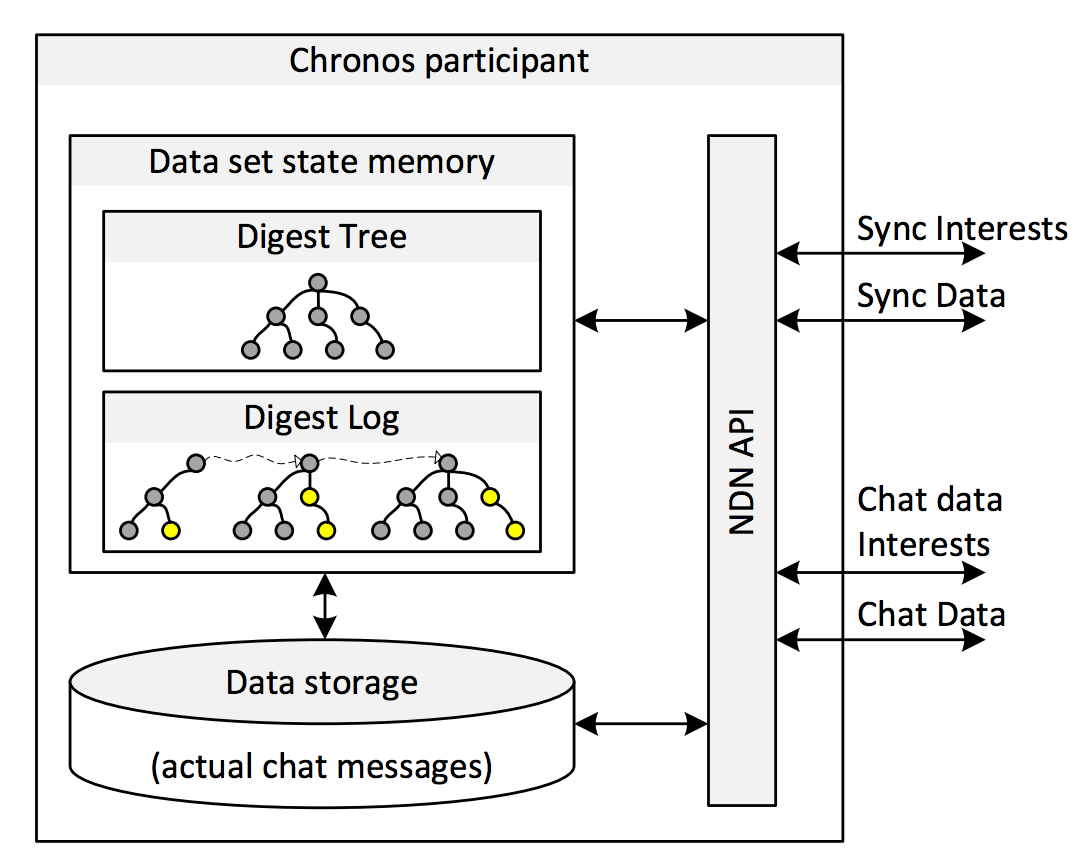
\includegraphics[width=4.5in]{png/digest.png}
\caption{ChronoSync中得摘要树和摘要记录}
\end{figure}

任何ChronoSync的应用程序的核心是两个相互依存的组件。
同步的数据集的状态的ChronoSync模块,
和响应该数据集的状态的变化的应用逻辑模块。
在ChronoChat ,ChronoSync模块以一个摘要树的形式保持当前用户的所有邮件知识。
在一个摘要日志的形式的数据集的状态变化。
当ChronoSync模块发现聊天室有新的消息,它会通知ChronoChat逻辑模块来获取和存储的消息。

为了发现数据集的变化,ChronoSync模块向
每个ChronoChat实例发送一个同步的兴趣,
其名称中包含的状态摘要,并将此状态维持在根摘要树。
通常,通过摘要树和摘要日志的帮助,ChronoSync可以直接推断数据集的更改,
以及与包含数据回复到同步感兴趣的变化,这是称为同步数据。

Chronosync仅仅着眼于促进有关在数据集中的新数据项的同步,
具体知道了同步信息后做什么是应用程序的工作。
例如,在ChronoChat同步数据带回消息的名字新添加到聊天室,
因而使用者的知识该数据集是带来最新。
然而,用户可 决定是否要取回所有丢失的信息,或只取回最近期的。

\begin{figure}
\centering
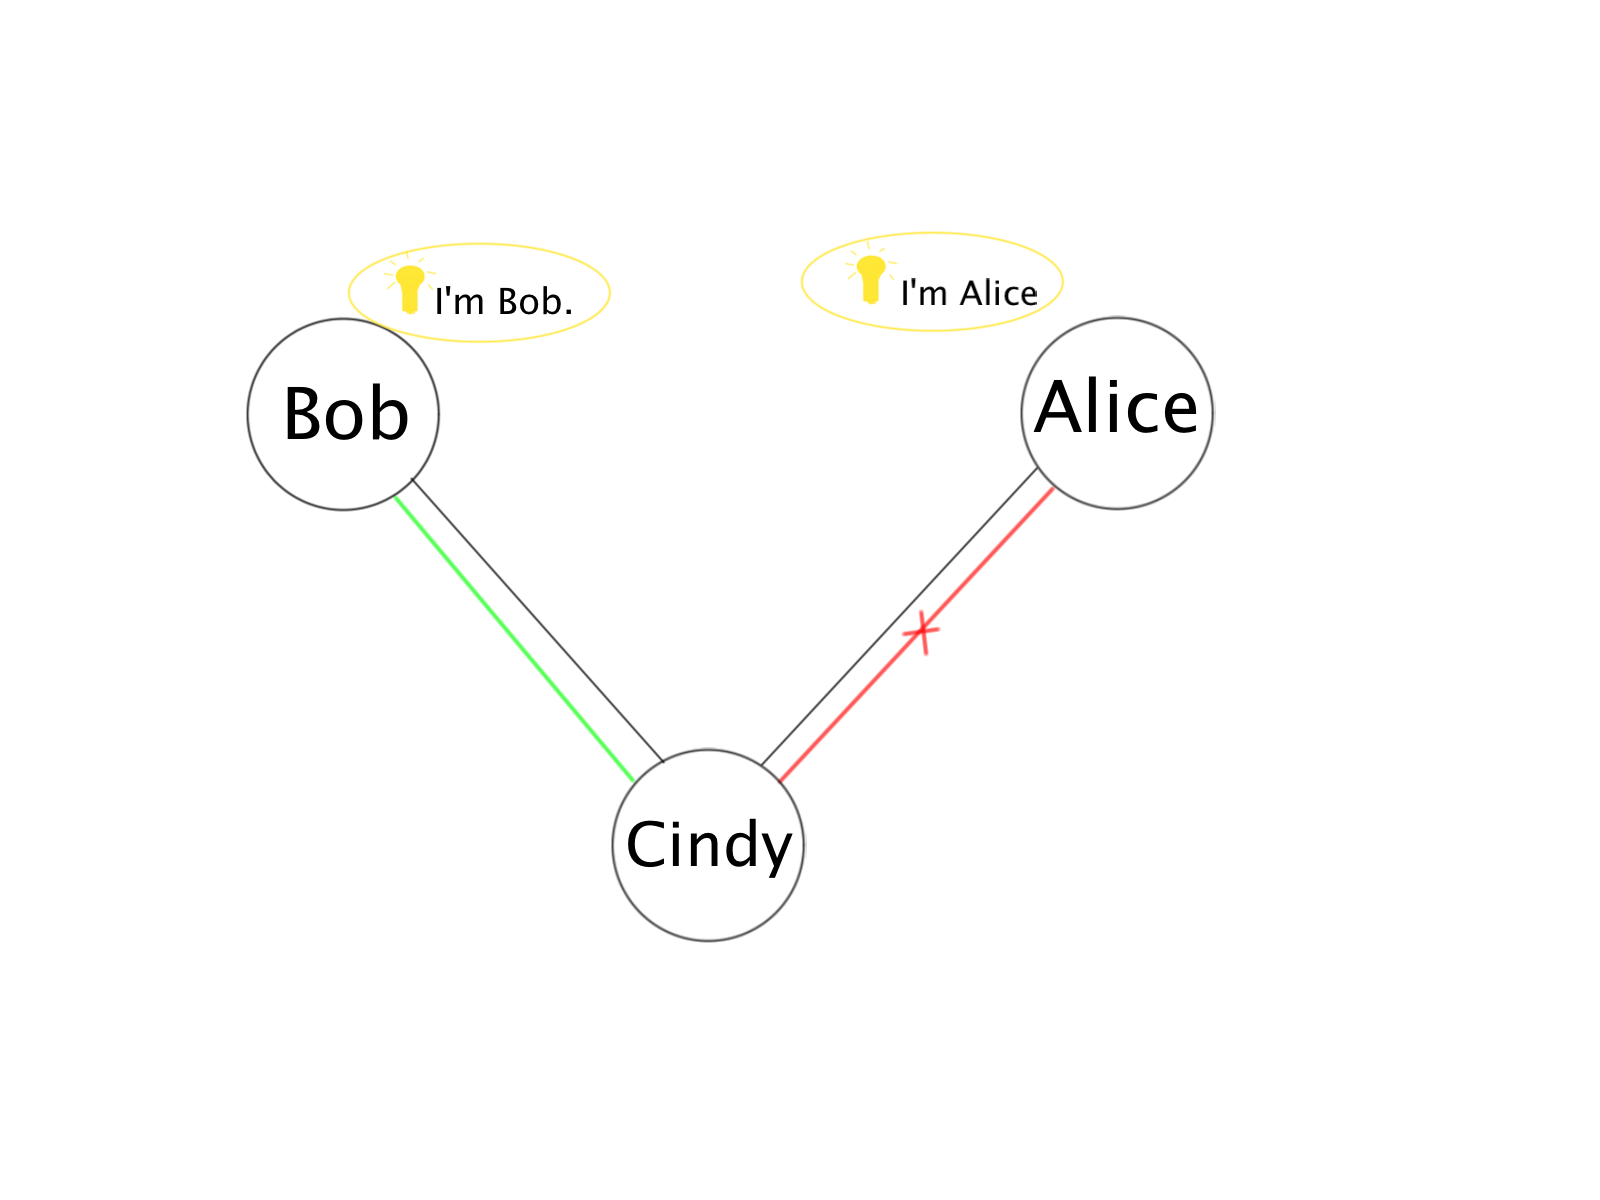
\includegraphics[width=4.5in]{png/simultaneous.png}
\caption{Simultaneous Message Generation Problem on ChronoSync}
\label{simultaneous}
\end{figure}

ChronoSync的主要缺点是控制能力,其短,
导致的问题来处理频繁的同步数据的产生。
当这种情况发生时,系统将被分成两个不同的组,并且不能识别来自彼此消化。
例如,如图\ref{simultaneous}所示,
Cindy发出同步的兴趣,要求谁产生一个最新的消息。
如果Alice和Bob说一些在接近的时间,也就是说,
Alice说些什么之前,Bob的话达到Cindy。
在这种方式下,爱丽丝将响应Cindy的同步兴趣,
但它永远不会达到Cindy因为从Cindy同步的兴趣只能取一个数据早在NDN 。
在这个时候,Bob和Cindy都在同一个状态,但Alice是没有的。
本系统被分为两个组,可以不相互识别。

\begin{figure}
\centering
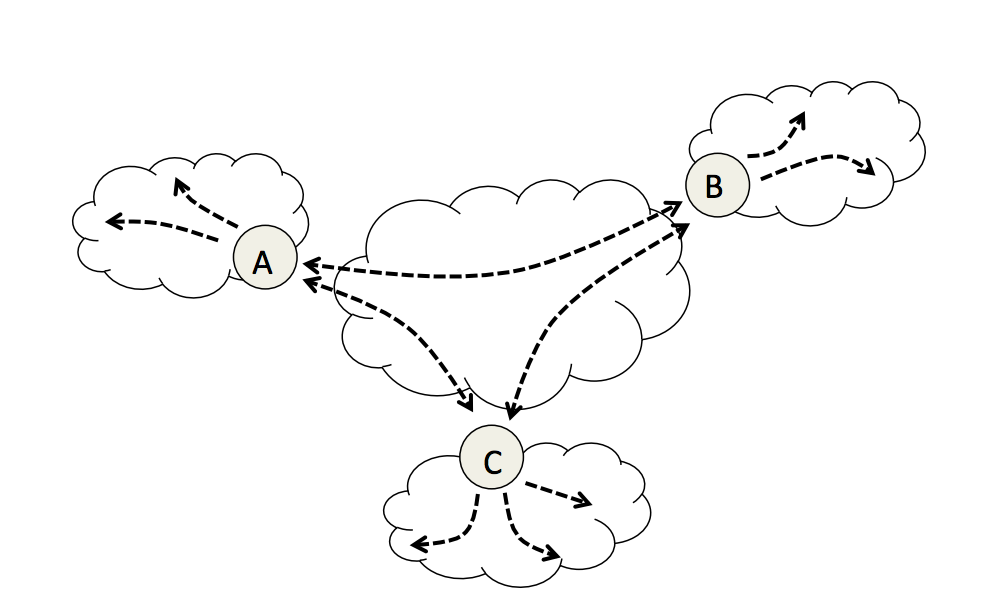
\includegraphics[width=4.5in]{png/chronosync_overlay.png}
\caption{Simultaneous Message Generation Problem on ChronoSync}
\label{simultaneous}
\end{figure}

另外一个不足是它不具备可扩展性,只能在较小的范围内使用.
由于没有层级结构,每次发送兴趣包都是要向全网广播,这导致了这种算法不能使用在较大的拓扑结构中.
只能在两个相距较远的组之间建立一个覆盖层,并通过这个隧道进行通讯.
